\documentclass[11pt]{standalone}
\usepackage{tikz}

\begin{document}

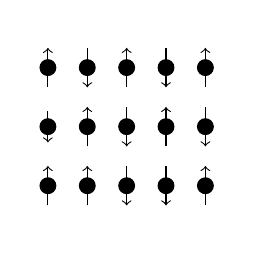
\begin{tikzpicture}
% The below code can be looped and shortened!
\draw[fill=black] (0,0) circle (.1cm);% node[](9){};
\draw[fill=black] (-0.5,0) circle (.1cm);
\draw[fill=black] (-1.0,0) circle (.1cm);
\draw[fill=black] (0.5,0) circle (.1cm);
\draw[fill=black] (1.0,0) circle (.1cm);

\draw[fill=black] (0,0.75) circle (.1cm);
\draw[fill=black] (-0.5,0.75) circle (.1cm);
\draw[fill=black] (-1.0,0.75) circle (.1cm);
\draw[fill=black] (0.5,0.75) circle (.1cm);
\draw[fill=black] (1.0,0.75) circle (.1cm);

\draw[fill=black] (0,-0.75) circle (.1cm);
\draw[fill=black] (-0.5,-0.75) circle (.1cm);
\draw[fill=black] (-1.0,-0.75) circle (.1cm);
\draw[fill=black] (0.5,-0.75) circle (.1cm);
\draw[fill=black] (1.0,-0.75) circle (.1cm);

% Spins
\draw[<-] (-1,-0.2) -- (-1,0.2);
\draw[->] (-0.5,-0.25) -- (-0.5,0.25);
\draw[<-] (0,-0.25) -- (0,0.25);
\draw[<-] (1,-0.25) -- (1,0.25);
\draw[->] (0.5,-0.25) -- (0.5,0.25);

\draw[<-] (-1,1) -- (-1,0.5);
\draw[->] (-0.5,1) -- (-0.5,0.5);
\draw[<-] (0,1) -- (0,0.5);
\draw[<-] (1,1) -- (1,0.5);
\draw[->] (0.5,1) -- (0.5,0.5);

\draw[->] (-1,-1) -- (-1,-0.5);
\draw[->] (-0.5,-1) -- (-0.5,-0.5);
\draw[<-] (0,-1) -- (0,-0.5);
\draw[->] (1,-1) -- (1,-0.5);
\draw[<-] (0.5,-1) -- (0.5,-0.5);


% Blanks
\draw[<->, color=white] (-1.25,1.25) -- (-1.25,-1.25);
\draw[<->, color=white] (1.25,0.35) -- (1.25,-0.35);

\end{tikzpicture}

\end{document}